\chapter{Introduktion}
Vi vil indledningsvis præsentere konteksten for dette speciale. Herefter klarlægger vi, hvilke problemer vi ønsker at berøre samt hvad vores tilgangsvinkel er. Afslutningsvis giver vi et overblik over specialets struktur. 

\section{Kontekst}
Over de sidste par år er multi-kerne cpu'er blevet hyldevarer, hvilket har afledt et stigende behov for at udvikle programmer, der kan udnytte flere kerner samtidigt. Dette behov har gjort CSP til et populært sprog, da det gør det let at repræsentere samtidighed og desuden kræver eksplicit udveksling af data frem for at benytte delte datastrukturer, som kræver låsemekanismer eller anden form for kontrol over hvem der tilgår og hvordan det delte data tilgås. CSP's stigende popularitet har affødt at det er blevet blevet implementeret i flere andre programmeringssprog, og senest har Google lavet sproget Go, der er baseret på CSP. 

Tid har altid været et brugbart værktøj indenfor datalogi, men har ofte været besværligt at repræsentere og håndtere. Det har ført til megen forskning og udvikling indenfor området, og har resulteret i adskillige modeller og frameworks. I den forbindelse er der også lavet en model for tid i CSP, kaldet TimedCSP. Dette er hovedsageligt et teoretisk arbejde som aldrig har vundet indpas i nogle af de gængse implementation af CSP. Der er derfor, så vidt vi ved, på nuværende tidspunkt ikke nogen gængs anvendt implementation af tid i CSP. 

\inline{ Jeg synes vi skal motivere for tid uafhængigt af pycsp,  og så i et tredje afsnit sige at tilsammen vil det være rigtig smart. Så 1. pycsp er smart (er skrevet). 2 tid er smart (mangler). 3 tilsammen er det rigtig smart (skal omskrives), baseret på Brians motivering d. 3 maj}
\fxnote{RS: Jeg har lavet udkast, du kan prøve at kaste flere ord efter det hvis du lyster}
\section{Specialets problemformulering og struktur}
Set i lyset af den nuværende mangel på en praktisk anvendelig implementering af tid i CSP, vil vi undersøge om det er muligt at lave en sådan - dvs. en implementering, som kan bruges af udviklere til at løse problemer, hvori tid indgår.

For at opnå dette vil vi undersøge, hvad der skal til for at introducere følgende tre anvendelsesområder i \pycsp: Diskret simulering, realtids planlægning og interaktiv planlægning. Disse anvendelsesområder repræsenterer områder hvor tid indgår  og dækker tilsammen bredt over tid som helhed. Diskret simulering anvendes i stor udstrækning i discrete event simulation. Realtids planlægning benyttes i tidskritiske systemer hvor der er stringente krav om at en given begivenhed er blevet udført inden for en tidsramme. Endeligt bruges interaktiv planlægning i spilindustrien til at udregne scenen i et computerspil. På \cref{fig:intro} viser vi hvordan vi forventer at kombinere anvendelsområderne med \pycsp for derved at komme frem til vores Timed \pycsp. 

\begin{figure}[htp]
 \begin{center}
  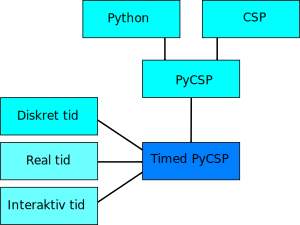
\includegraphics[scale=0.8]{images/intro}
	\caption{Samspil mellem CSP, Python og de tre anvendelsområder af tid samlet i Timed \pycsp .}
	\label{fig:intro}
\end{center}
\end{figure}

For hver model vil vi definere en række eksempler, der illustrerer disse anvendelsesområderne. Eksemplerne skal sikre den praktiske anvendelighed og senere bruges til at vise, hvordan et tidsspecifikt problem kan løses henholdsvis med og uden vores udvidelse. Eksemplernes formål er altså, at give et klart indblik i de krav, der stilles til en udvidelse af \pycsp, og hvilke fordele en introduktion af de givne anvendelsesområderne i \pycsp vil give. På denne baggrund vil vi komme med løsningsforslag som tager udgangspunkt i den praktiske anvendelighed. Disse løsningsforslag vil såfremt det er muligt, blive implementeret som en udvidelse af \pycsp.

Specialet vil derfor være struktureret som følger. I \autoref{chap:csp} vil vi gennemgå CSP og \pycsp med fokus på de dele der er relevante i forhold til at introducere tid. I \autorefs{chap:des}, \ref{chap:rtp} og \ref{chap:is} vil vi gennemgå de tre anvendelsesområder som beskrevet ovenfor. Afslutningsvis vil vi foretage en samlet i evaluering og konklusion i \autoref{chap:konklusion} på baggrund af delkonklusionerne i \autorefs{chap:des}, \ref{chap:rtp} og \ref{chap:is}.

%Mål: At lave en praktisk anvendelig udviddelse af pycsp, som kan bruges af udviklere til at løse problemer, der har en naturlig dimension af tid.

%Mål: At undersøge om det er muligt at lave en praktisk anvendelig udviddelse af pycsp, som kan bruges af udviklere til at løse problemer, der har en naturlig dimension af tid.

\section{Vores bidrag}
\section{Termer}

%\item I \des beskriver det enkelte \code{event} en begivenhed, og vi vil i dette speciale bruge ordet begivenhed for en event i \des. 
%\item simulering ikke simulation
%\item implementering ikke implementation.
%\item event: begivenhed
%\item Vi har fra koden der vises fjernet kode der ikke er relevant for sammenhængen, som f.eks kald til logging. Linje nr. vil derfor ikke altid passe, men det første linje nr i kodestumpen vil svare til linjenr i source koden.
%\item TODO: vi skal søge og styr på  greenlet vs. greenlets
%\item søg igennem grenelts og varianter
%\item SKIP-guard, skip-guard \code{skip-guard}? træf et valg mht. både skip og timeout. 

\begin{list}{}{}
\item \textbf{\Sched} dækker over det engelske ord Scheduler. En \sched~ er det software der står for at planlægge i hvilken rækkefølge processerne skal udføres på computeren.
%\item \textbf{Tidsdomænet} Tidsdomænet er den overordnede .... \fxwarning{Hvad fanden skal der stå her}
\item \textbf{Realtid} er en tidsmodel, der i litteraturen også er defineret som absolut tid, eller Newtonisk tid. Tiden ses som en fundamental struktur i universet, der 
fremskrives kontinuerligt og uafhængigt af nogle eksterne kræfter.
\item \textbf{Diskret tid} er en anden tidsmodel. Her samples værdier fra den kontinuerlige tid, således at tiden fremskrives i ryk. Den enkelte samples er normal taget med et konstant tidsinterval, men kan også være taget med et variable tidsinterval. I diskret tid kan tiden enten drives frem af tiden selv som i realtid, eller at den manuelt  skal fremskrives. I dette speciale defineres diskret tid til at have variable tidsinterval, og skal fremskrives mauelt.
\item \textbf{Anvendelsesområde} er en konkredt implementation af en tidsmodel.
\item \textbf{\code{Skrivemaskine-font}} markerer i dette speciale de  variabelnavne, funktioner,  klasser og moduler  der er  der er specifikt for Python.
\end{list}



